\documentclass[11pt]{article}
\pagestyle{plain}

\usepackage{amssymb}
\usepackage{amsmath}
\usepackage{amsfonts}
\usepackage{graphics}
\usepackage{graphicx}
\usepackage[margin=1in]{geometry}
\usepackage{svg}
\usepackage{float}

\title{LINMA1170 - Devoir 2}
\author{Giovanni Karra - 45032100}

\begin{document}

\maketitle

\section*{Question 1}
Nous souhaitons étudier la sensibilité de la solution d'un problème par rapport à des perturbations dans l'entrée. Le nombre de conditionnement $\kappa$ d'un problème est la borne supérieur du ratio entre la perturbation relative de la solution et celle introduite dans l'entrée. \\
Plus formellement, si on considère une fonction $f$ comme la solution et $x$ comme l'entrée, nous avons :
\begin{align}
    \kappa = \sup_{\delta x}\left. \frac{||\delta f||}{||f||} \middle/ \frac{||\delta x||}{||x||} \right.
\end{align}
Il est important de préciser que le conditionnement s'applique uniquement les propriétés mathématiques d'un problème, et non pas la perturbation causée par un algorithme qui résout le problème (voir \textit{stabilité}).\\
Pour le problème des moindres carrées, cette borne peut être facilement calculée avec deux formules\footnote{cf Trefethen page 129 pour la démonstration} qui donnent le nombre de conditionnement selon $A$ et selon $b$ respectivement :
\begin{align}
    \kappa_b = \frac{\kappa(A)}{\eta \cos(\theta)}~~~~~~~\kappa_A = \kappa(A) + \frac{\kappa(A)^2\tan(\theta)}{\eta}
\end{align}
avec
\begin{align}
    y = Ax ~~~ \eta = \frac{||A||||x||}{||y||} ~~~
    \theta = \arccos\left(\frac{||y||}{||b||}\right)
\end{align}
Pour vérifier cette borne numériquement, il suffit de générer des perturbations de différentes tailles, et de plotter la norme relative de la perturbation de l'entrée contre celle de la solution, comme nous pouvons le voir ci-dessous.
\begin{figure}[H]
    \centering
    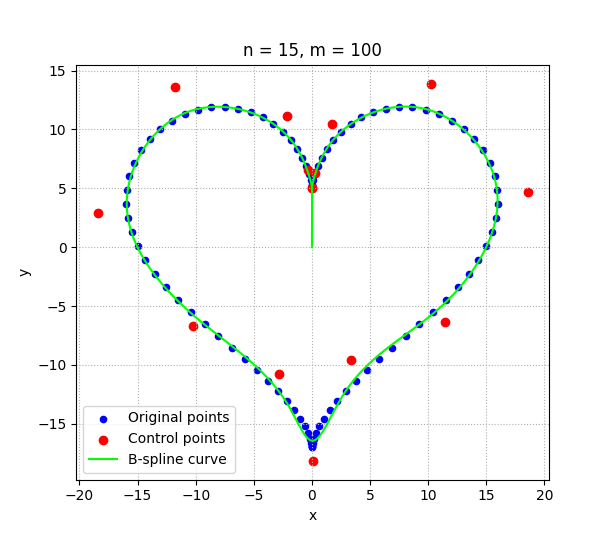
\includegraphics[scale=0.5]{../../Devoir1/rapport/images/coeur1.png}
    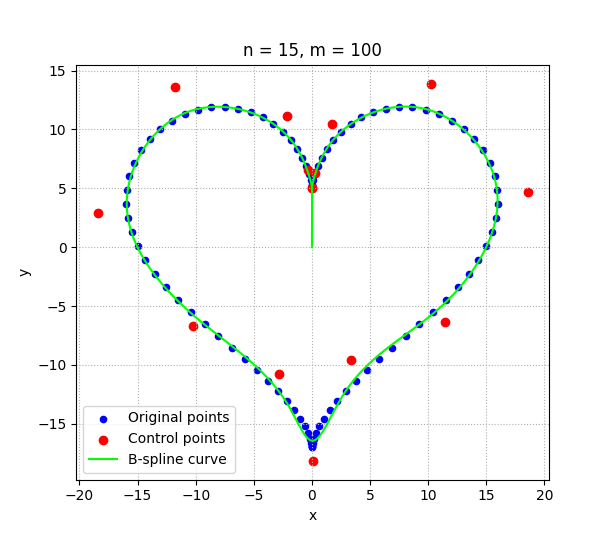
\includegraphics[scale=0.5]{../../Devoir1/rapport/images/coeur1.png}
    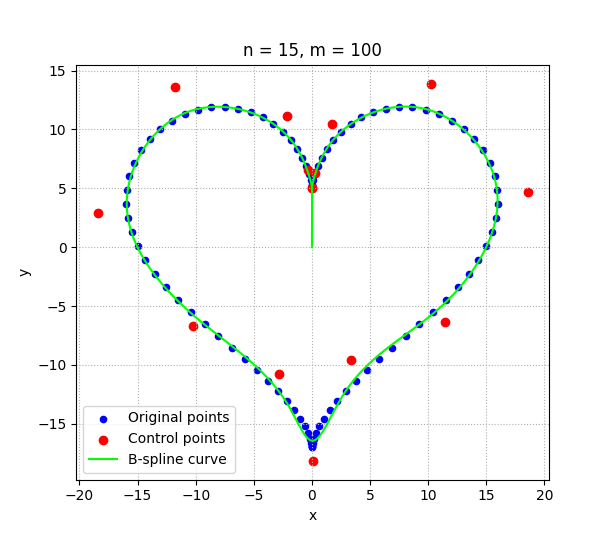
\includegraphics[scale=0.5]{../../Devoir1/rapport/images/coeur1.png}
    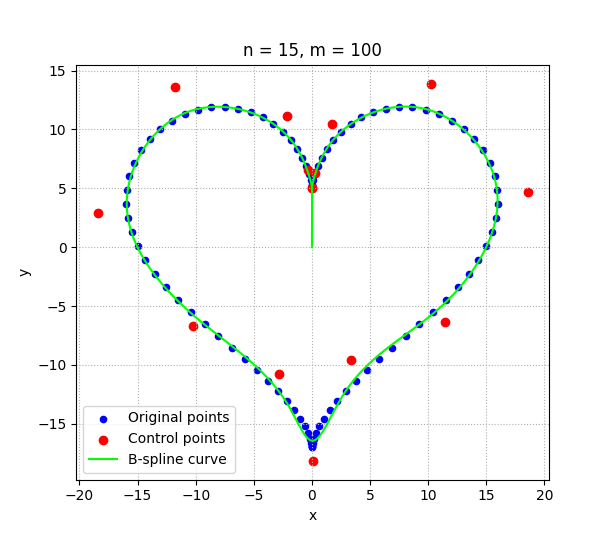
\includegraphics[scale=0.5]{../../Devoir1/rapport/images/coeur1.png}
\end{figure}
Nous pouvons voir que la perturbation empirique de la solution ne dépasse jamais la borne calculée mathématiquement.


\section*{Question 2}
La complexité temporelle de l'algorithme de décomposition $LU$ est de $\mathcal{O}(\frac{2}{3}m^3)$, $m$ étant le nombre de lignes/colonnes de la matrice carrée de départ.\\
Cet algorithme n'est pas facilement parallélisable, car les opérations sur les lignes dépendent des opérations réalisées sur les lignes précédentes.


\section*{Question 3}
Soit $A_k$ la matrice carrée $k\times k$ tel que tous ses mineurs principaux sont positifs, et $A_k^{elim}$ cette même matrice après avoir subit une élimination gaussienne.\\
Supposons que la matrice $A_k$ n'ait pas besoin de pivotage lors de sa décomposition $LU$, et prouvons que c'est le cas aussi pour $A_{k+1}$.\\
\begin{align}
    A_{k+1} = \left[\begin{array}{cc}
        A_k & v\\
        w^T & a_{k+1k+1}
    \end{array}\right] ~~~ \Rightarrow ~~~
    A_{k+1}^{elim} = \left[\begin{array}{cc}
        A_k^{elim} & v'\\
        0 & a_{k+1k+1} - C
    \end{array}\right]
\end{align}
Pour montrer qu'il n'y a pas besoin de pivotage, il suffit de montrer que $a_{k+1k+1} - C$ est positif.\\
Nous savons que le déterminant d'une matrice de change pas après une soustraction de lignes. Nous savons aussi par l'expansion de Laplace que le déterminant d'une matrice peut être exprimé comme suit :
\begin{align}
    \det(A) = \sum_{j=1}^{n}a_{ij}(-1)^{i+j}M_{ij}
\end{align}
Où $i$ est une ligne fixée, et $M_{ij}$ le déterminant de la sous-matrice obtenue en retirant la ligne $i$ et la colonne $j$. En appliquant l'expansion de Laplace à $A_{k+1}^{elim}$ en fixant $i$ à $k+1$, nous obtenons :
\begin{align}
    \det(A_{k+1}^{elim}) = a^{elim}_{k+1k+1}(-1)^{2(k+1)}\det(A_k^{elim}) = a^{elim}_{k+1k+1}\det(A_k^{elim}) > 0
\end{align}
Les autres éléments de la dernière ligne sont nuls, et nous savons que $\det(A_{k+1}^{elim}) > 0$ grâce au postulat de départ. Nous savons que $\det(A_k^{elim}) > 0$, donc pour que $(6)$ soit vérifiée, nous devons nécessairement avoir $a^{elim}_{k+1k+1} = a_{k+1k+1} - C > 0$, et donc nous n'avons pas besoin de pivoter.\\\\
Démontrons un cas de base avec
\begin{align}
    A_k = \left[\begin{array}{cc}
        a & b\\
        c & d
    \end{array}\right], ~~~ a > 0, ~~~ d > 0, ~~~ \det(A) = ad - bc > 0
\end{align}
En appliquant l'élimination gaussienne, nous obtenons
\begin{align}
    A_k = \left[\begin{array}{cc}
        a & b\\
        0 & d - \frac{bc}{a}
    \end{array}\right] =
    \left[\begin{array}{cc}
        a & b\\
        0 & \frac{ad - bc}{a}
    \end{array}\right] = 
    \left[\begin{array}{cc}
        a & b\\
        0 & \frac{\det(A)}{a}
    \end{array}\right]
\end{align}
Nous savons que $a_{22}$ est positif car $a > 0$ et $\det(A) > 0$.\\
Par recurrence, nous pouvons affirmer que cette propriétés s'applique à toutes les matrices dont les mineurs principaux sont positifs.\\
Cela inclu bien-sûr la matrice $A^TA$ de l'équation normale, car c'est une matrice symétrique et définie positive, ce qui est une condition équivalente à avoir tous les mineurs principaux positifs.

\section*{Question 4}
Résoudre un problème des moindres carrés revient à resoudre l'équation normale, c'est-à-dire résoudre le système d'équations
\begin{align}
    \tilde{A}x = \tilde{b}
\end{align}
avec
\begin{align}
    \tilde{A} = A^TA ~~~~~~~~~~~ \tilde{b} = A^Tb
\end{align}
Au lieu d'utiliser la décomposition $LU$ pour résoudre ce système, nous pouvons utiliser la factorisation de Cholesky, qui exploite la symétrie et la définie-positivité de $\tilde{A}$ pour accélérer le processus. En effet, la factorisation de Cholesky utilise en théorie deux fois moins d'opérations que la décomposition $LU$, et nous pouvons vérifier ceci empiriquement sur les figures ci-dessous.
\begin{figure}[H]
    \centering
    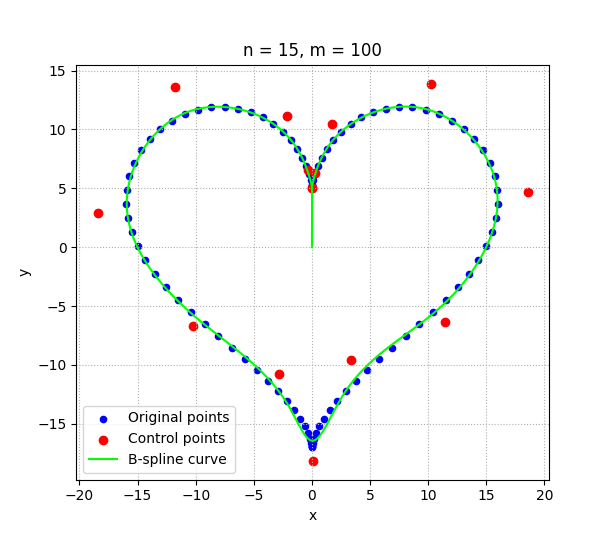
\includegraphics[scale=0.5]{../../Devoir1/rapport/images/coeur1.png}
    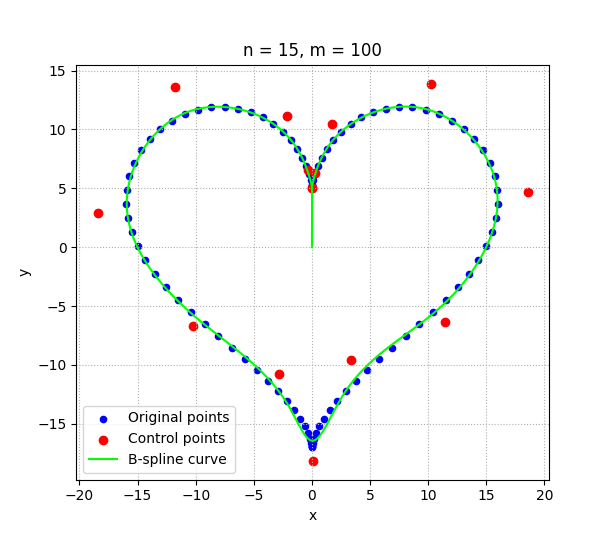
\includegraphics[scale=0.5]{../../Devoir1/rapport/images/coeur1.png}
\end{figure}

\end{document}